\documentclass{arduino}
\setmainlanguage{croatian}

\begin{document}

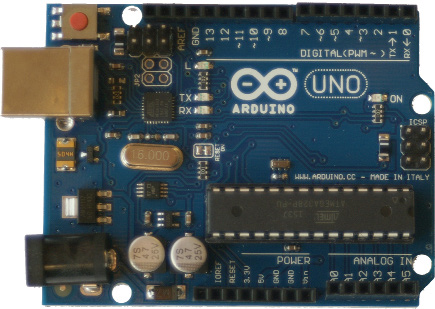
\includegraphics[width=\linewidth]{1. Arduino}

\textbf{Zahtjevi za ovaj modul}

\begin{tabular}{
    @{}>{\raggedright\arraybackslash}p{0.5\linewidth-\tabcolsep}
    >{\raggedright\arraybackslash}p{0.5\linewidth-\tabcolsep}@{}
}
\textbf{Izvanmrežno}                                                                  & \textbf{Na liniji} \\
Arduino                                                                           & ---             \\
Breadboard                                                                        & ---             \\
Džemper kabeli                                                                     & ---             \\
Otpornici (\SI{220}{\ohm}; \SI{330}{\ohm}; \SI{1}{\kilo\ohm}; \SI{10}{\kilo\ohm}) & ---             \\
Potenciometar (\SI{1}{\kilo\ohm}; \SI{10}{\kilo\ohm})                             & ---             \\
Dioda                                                                             & ---             \\
2x LDR                                                                            & ---             \\
LED (crvena, žuta, zelena)                                                          & ---             \\
RGB LED                                                                           & ---             \\
Servo motor                                                                       & ---             \\
Istosmjerni motor                                                                          & ---             \\
5x Pritisnite tipku                                                                    & ---             \\
2N2222 tranzistor                                                                 & ---             \\
LCD                                                                               & ---             \\
Aktivni piezo element                                                              & ---             \\
\end{tabular}

\textbf{Preduvjet znanja}

\begin{tabular}{@{}ll@{}}
Ohmov zakon                                                 &  $R = \dfrac{U}{I}$            \\
Komponente u serijama                                      &  jednaka struja                 \\
Komponente paralelno                                   &  jednak napon                 \\
Vlast                                                     &  $P = U \cdot I = I^2 \cdot R$ \\
\multicolumn{2}{@{}l@{}}{Rad alternatora / elektromotora} \\
\end{tabular}

\newpage

\section{Uvod}

\marginfigure[\baselineskip]{2. Aurduino - welcome}
Lijepo što započinjete s Arduinom! Možda nemate pojma što je Arduino i što s njim možete učiniti. Arduino je vrsta mikroračunala. Arduino možete povezati s računalom odakle šaljete program (u Arduinu to nazivaju skicom) na Arduino. Tada će Arduino pokrenuti vašu napisanu skriptu i pobrinuti se za izlaz. Na primjer, možete držati hladnjak na određenoj temperaturi, kontrolirati samovozećeg robota, izraditi svjetlosne senzore, kontrolirati LCD zaslon na košulji i tako dalje. Također je moguće ne koristiti softver i igrati se samo s elektronikom. Tada je Arduino izvor napona.

U ovom modulu radit ćemo s Arduinom i naučiti osnovne mogućnosti Arduina. Kada radite s Arduinom, imate dva važna dijela: Arduino i ploču za ploču. Arduino je računalo s ulaznim i izlaznim mogućnostima. Na ploču spajate elektroniku kojom upravlja Arduino.

\subsection{Breadboard}

\marginfigure[\baselineskip]{3. Arduino - breadboard}
\marginfigure[\baselineskip][0.5]{4. Breadboard}
Ploča s dvije strane ima dva stupca koja su spojena na napajanje (+ i -). + Strana je spojena na \SI{5}{\volt} izlaz ili na izlazni port Arduina. Bočna strana spojena je na GND (tlo) Arduina. Iako ne koristite uvijek stalni izlaz, pametno ga je uvijek povezati.

Zaslon ima redove i stupce. Slika s desne strane prikazuje pločicu, a ispod nje vidite kako se interno povezuju. Točke u nizu su povezane. Ali nemojmo se predugo zadržavati na ovome\dots Započnimo!

\textbf{NOTE:} Često morate navesti na koji je USB priključak vaš Arduino povezan s računalom. To radite odlaskom u program na: Tools / Port. Tamo možete kliknuti na ispravni USB priključak.

\newpage

\subsection{Zadatak 1 Spajanje LED diode}

\marginpar{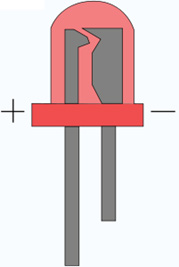
\includegraphics[width=0.3\linewidth]{5. Component LED}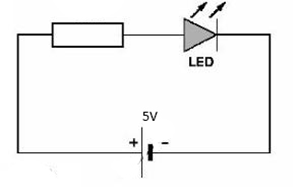
\includegraphics[width=0.7\linewidth]{6. LED circuit}}
LED je dioda koja emitira svjetlost kad kroz LED teče struja. LED omogućuje protok struje samo u jednom smjeru. Duga noga LED-a uvijek mora biti povezana sa + stranicom, kratka noga sa bočnom stranom, pogledajte sliku sa strane.

Struja kroz LED obično može biti samo \SI{20}{\milli\ampere}. Tada je napon na LED diodi približno \SI{2.0}{\volt}, ove se vrijednosti malo razlikuju po vrsti LED-a, pogledajte donju tablicu. Arduino isporučuje a \SI{5.0}{\volt} napon. LED dioda stoga mora biti povezana u seriju s otpornikom. Otpor stoga mora biti najmanje \SI{150}{\ohm} ($R = \frac{U}{I} = \frac{\SI{3.0}{\volt}}{\SI{0.020}{\ampere}} = \SI{150}{\ohm}$).


\marginfigure[\baselineskip]{8. Circuit switchable LED}
\begin{alphalist}
\item Nema otpornika s \SI{150}{\ohm}, ali postoji jedan od \SI{220}{\ohm}. Potražite otpor pomoću koda boje: prvi prsten mora biti crven, drugi prsten također i treći prsten smeđi ($\textcolor{red}{2}\textcolor{red}{2} \cdot \textcolor{brown}{10}$). Druga mogućnost je crvena, crvena, crna, crna ($\textcolor{red}{2}\textcolor{red}{2}\textcolor{black}{0} \cdot \textcolor{black}{1}$).

\item Sada spojite \SI{5}{\volt} izlaz Arduina na + stupac i GND (zemaljski) izlaz Arduina na - stupac.

\item Spojite LED i otpornik u seriju, pogledajte crtež.

\item Spojite Arduino na računalo putem USB-a. Ako ste to učinili ispravno, LED će svijetliti!
\end{alphalist}

Budući da crvena LED svjetlost emitira na nižem naponu od, primjerice, zelene LED, možete upotrijebiti manji otpor za zelene i plave LED diode. Na taj način izgaraju jednako jako!

\begin{tabular}{ll}
\textbf{Boja} & \textbf{Prag napona} \\
Plava            & \SI{2.3}{\volt}            \\
Zelena           & \SI{2.0}{\volt}            \\
Crvena             & \SI{1.5}{\volt}            \\
\end{tabular}

\begin{minipage}[t]{\linewidth}
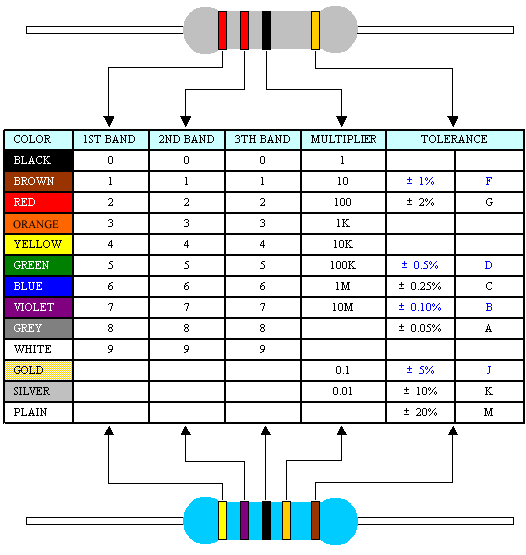
\includegraphics[width=0.8\linewidth]{7. Component resistor values (EN)}
\end{minipage}

\newpage
\subsection{Zadatak 2 Trepćuća LED dioda}

\marginfigure[\baselineskip]{9. Circuit blinking LED}
\marginfigure[\baselineskip]{8. Circuit switchable LED}

Sada možete upaliti LED diodu, ali to vam još neće biti od velike koristi\dots Sljedeći je korak upravljanje LED diodom pomoću dijela koda. Za kontrolu LED diode pomoću koda potrebno je spojiti izlazni priključak (na primjer pin 13) Arduina na LED diodu. Ne trebate \SI{5}{\volt} izlaz sada, pin 13 sada daje napon. Na crtežu možete vidjeti da \SI{5}{\volt} izlaz je i dalje povezan. S većim projektima brzo zaboravljate \SI{5}{\volt}, zato je pametno uvijek ga povezati!

\begin{alphalist}
\item Izgradite postavke koje vidite na crtežu i spojite Arduino na računalo.
\end{alphalist}

Želimo kontrolirati Arduino, za to koristimo program Arduino.

\begin{alphalist}
\item Otvorite program i otvorite treptanje skripte putem: file / examples / base / blink.

\item Provjerite skriptu kvačicom. Ako program ne radi, na dnu će prikazati poruku o pogrešci (možda ćete morati dodijeliti COM priključak, to radite putem alata / porta).

\item Prenesite skriptu na svoj Arduino pomoću gumba 
\includegraphics{10. Arduino upload} (shortcut: ctrl + u)

\item Ukratko opišite ono što vidite. Pokušajte objasniti što vidite pomoću koda.

\item Promijenite skriptu tako da LED brže treperi.

\item Spojite tri različita LED svjetla, promijenite skriptu tako da se uzastopno uključuju.

\item Promijenite skriptu i nakratko stvorite semafor s uključenom narančastom bojom.
\end{alphalist}

\newpage

\begin{widebox}
    \begin{leftrightbox}[0.4]{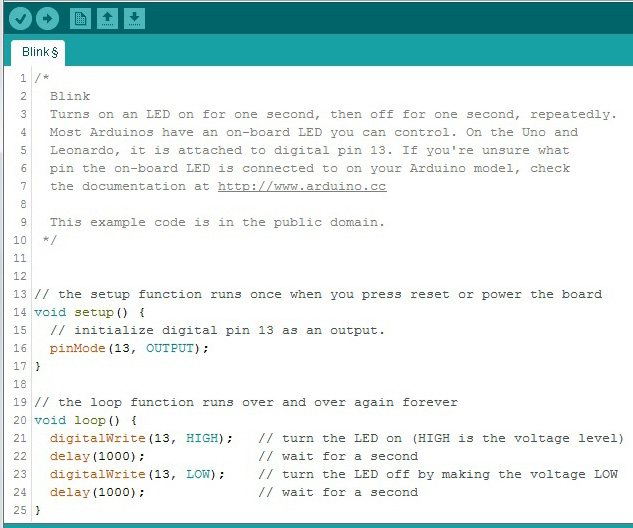
\includegraphics[width=\linewidth]{12. Arduino code}}
    \section{Programiranje 1. dijela}

    Arduino ima vlastiti programski jezik zasnovan na C ++. Ako već imate iskustva s programiranjem i / ili sa C ++ (ili Javom), programiranje je vrlo jednostavno. A ako nemate iskustva s programiranjem? Puno je manje teško nego što možda mislite!

    Na vrhu skripte Blink prvi znak je / *, što znači da se komentira sve nakon ovog početnog znaka i prije završnog znaka * /. Kôd između ovih znakova program zanemaruje. Ovdje stavljate naziv programa, ono što radi, tko ga je napravio i kada ste ga zadnji put promijenili.
    \end{leftrightbox}
\end{widebox}

\smallskip

Druga mogućnost dodavanja komentara je uz pomoć //. Sve u istoj liniji nakon // je komentar. Na taj način možete pratiti što kôd radi na toj liniji. Pomoću prečaca ctrl + / možete brzo komentirati cijeli redak koda.
\begin{marginlisting}
void setup(){
  pinMode(13,OUTPUT);
}
\end{marginlisting}

Prije izvršavanja najvažnijeg koda morate reći što se točno kontrolira. Prvo kažemo Arduinu da postoji nešto na pinu 13 i da bi Arduino trebao dati izlaz (napon). Bilo bi malo urednije prvo definirati ime pina 13 prije postavljanja: pinu dajete ime (\lstinline{int LEDred = 13;}). Ako tada želite kontrolirati pin 13, to možete učiniti s imenom LEDred.
\begin{marginlisting}
void loop() {
  digitalWrite(13, HIGH);
  delay(1000);
  digitalWrite(13, LOW);
  delay(1000);
}
\end{marginlisting}

Sve između kovrčavih zagrada \{\} petlje ponavlja se kontinuirano. Prva iglica 13 napravljena je visoko (\SI{5.0}{\volt}) pomoću koda \lstinline{digitalWrite} (\lstinline{digitalWrite} može biti samo uključeno ili isključeno). Tada program mora pričekati \SI{1000}{\milli\s} prije izvođenja sljedećeg retka koda. Sljedeći redak koda opet čini pin 13 niskim (\SI{0.0}{\volt}). Tada program mora pričekati \SI{1000}{\milli\s} opet, prije nego što ponovno pokrene petlju.

\marginfigure[-3\baselineskip]{13. PWM}

Pin se kontrolira s visokim ili niskim signalom. Postoji li još nešto između? da i ne \dots Izlaz je uvijek \SI{0.0}{\volt} ili \SI{5.0}{\volt}. Ali LED možete zatamniti uključivanjem LED-a samo određeno vrijeme. Ako LED trepće dovoljno brzo, nećete vidjeti LED kako trepće, samo se čini da je LED slabije svijetli. Ako želite prigušiti LED, upotrijebite izlaz sa simbolom $\sim$. Ovo je modulacija širine impulsa (PWM). Vrijednost PWM-a je između 0 (potpuno isključeno) i 255 (potpuno uključeno).
\newpage

\subsection{Zadatak 3 LED s mogućnošću zatamnjivanja}

\marginfigure[\baselineskip]{14. Circuit dimmable LED}

\begin{alphalist}
\item Izgradite postavke s desne strane. Za izlaz upotrijebite PWM pin, na primjer Pin 9 (imajte na umu da LED ne mora biti priključen na konstantni napon, napon sada napaja pin 9).

\item Otvorite skriptu Fade u primjerima / bazi i prenesite skriptu.

\item Opišite što vidite i pokušajte objasniti što se događa uz pomoć koda.

\item Promijenite kod tako da LED brže svijetli i brže se gasi. Imajte na umu da postoje dva načina! Isprobajte ih oboje.

\item \lstinline{analogWrite} koristi se u kodu. Prije smo koristili \lstinline{digitalWrite}. Objasnite zašto to sada nije moguće.
\end{alphalist}

\subsection{Zadatak 4 Gumb za uključivanje i isključivanje LED diode}

\marginfigure[\baselineskip]{15. Circuit LED button}

Sada možemo uključiti i isključiti LED uz pomoć koda, pa čak i prigušiti ga. Ali često želite i ručno uključiti i isključiti strujni krug. Za to nam je potreban gumb.

\begin{alphalist}
\item Izgradite sklop s desne strane. Obavezno koristite veliki otpor tako da isporučena struja bude ograničena, jer Arduino loše napaja velike struje.
\end{alphalist}

Ideja je sada da koristimo pin 2 kao INPUT. Pin 2 mjeri napon u toj točki (uspoređuje ga s \SI{0.0}{\volt}). To se radi s kodom \lstinline{digitalRead()}. Sada može izmjeriti visoki (\SI{5.0}{\volt}) ili niska (\SI{0.0}{\volt})signal. Analognim pinom kao što je A0 do A5 mogu se mjeriti i međuvrijednosti, s 10-bitnom razlučivosti. Pin 2 treba mjeriti napon samo kad se pritisne tipka.

\begin{alphalist}
\item Otvorite skriptu gumba putem primjera / digitalno i prenesite skriptu.

\item Pritisnite gumb i provjerite kada je LED lampica isključena i kada svijetli.

\item Prilagodite skriptu tako da funkcija gumba bude obrnuta.
\end{alphalist}

\marginfigure[-\baselineskip]{16. Button bounce}

\textbf{NOTE:} S gumbom se događa nešto posebno. Gumb ima takozvani Bounce. To znači da napon ne ide izravno iz \SI{0}{\volt} do \SI{5}{\volt} ali opet ide gore-dolje. To je zato što se u gumbu nalazi opruga koja ide gore-dolje. Kad koristite i čitate gumb, korisno je ugraditi odgodu\dots

\newpage

\section{Programiranje 2. dijela}

Skripta gumba sveobuhvatnija je nego što smo vidjeli prije. Koračamo po koraku kroz skriptu.

\begin{marginlisting}
const int buttonPin = 2;
const int ledPin = 13;
\end{marginlisting}

Imamo posla s dvije pribadače na Arduinu gdje se nešto mora poduzeti. Pin 2 je ulaz, a pin 13 mora biti izlaz. Pin se ne mijenja, to je konstanta (\lstinline{const}). It is an integer value (\lstinline{int}). Dajemo pin 2 prepoznatljivo ime, pin 2 se sada naziva buttonPin. Pin 13 nazvan je ledPin.

\begin{marginlisting}
int buttonState = 0;
\end{marginlisting}

Uskoro ćemo htjeti znati kakvo je "stanje" gumba (pritisnuto ili ne). Može biti 1 ili 0. Prvo moramo reći Arduinu da želimo kasnije znati stanje gumba (stvoriti varijablu). Prije nego što pokrenemo skriptu, buttonState je jednako 0.

\begin{marginlisting}
void setup() {
  pinMode(ledPin, OUTPUT);
  pinMode(buttonPin, INPUT);
}
\end{marginlisting}

Kao što je spomenuto, moramo vam reći da je ledPin \lstinline{OUTPUT} a buttonPin je \lstinline{INPUT}. Sad to zna i Arduino\dots

Ali nešto se mora dogoditi kad se pritisne tipka. Na početku petlje očitava se gumb (zapravo mjeri se napon na otporu kako bi se vidjelo čita li \SI{5.0}{\volt}). Nakon toga an \lstinline{if} slijedi izjava. Ako (\lstinline{if}) the button is pressed (\lstinline{buttonState == HIGH}) tada bi LED trebao svijetliti (\lstinline{digitalWrite (ledPin, HIGH);}). U svim ostalim slučajevima (\lstinline{else}), LED ne smije svijetliti (\lstinline{digitalWrite (ledPin, LOW);}).

\begin{marginlisting}
void loop() {
  buttonState = digitalRead(buttonPin);
  if (buttonState == HIGH) {
    digitalWrite(ledPin, HIGH);
  }
  else {
    digitalWrite(ledPin, LOW);
  }
}
\end{marginlisting}

To je lako \lstinline{if} izjava. Također možete postaviti više uvjeta. Ako morate istovremeno pritisnuti dvije tipke prije nego što se LED upali, stavite \lstinline{&&} između likova (\lstinline{if buttonState1 == HIGH && buttonState 2 == HIGH)}).

Možete koristiti i lik \lstinline{||}. Tada se mora primjenjivati ​​jedan ili drugi uvjet. Nažalost, svjetlo još ne gori kad ste pritisnuli tipku. Ali možete promijeniti kôd kako biste bili sigurni da se svjetlo može paliti i gasiti jednim gumbom.

\begin{marginlisting}
void loop() {
  buttonState = digitalRead(buttonPin);
  if (buttonState == HIGH && state == LOW) {
    state2 = HIGH;
    }
  if (buttonState == HIGH && state == HIGH) {
    state2 = LOW;
    }
  state = state2;
  digitalWrite(ledPin,state);
  delay (100);
}
\end{marginlisting}

\begin{marginlisting}
if(buttonState == HIGH){i++;}
digitalWrite(ledPin,i%2);
\end{marginlisting}
Ne zaboravite definirati novu varijablu (\lstinline{int}) na početku! Postoje još jednostavniji načini, oni su prikazani samo kao skripta. Objasnite kako rade!

\begin{marginlisting}
digitalWrite(13,!digitalRead(13));
\end{marginlisting}

\newpage

\subsection{Zadatak 5 Osiguranje sefa}

Sef banke je osiguran. Sef se ne otvara (LED će svijetliti samo kad se okrenu dvije tipke (pritisnute tipke). Jedna ključanica nalazi se u upravnikovoj sobi, druga je pored sefa.

Izgradite odgovarajući krug i programirajte skriptu tako da se sef ne otvori dok se obje tipke istodobno ne okrenu.

\subsection{Zadatak 6 Dvosmjerna sklopka}

Kada ste na dnu stepenica želite upaliti svjetlo na vrhu stuba. Na vrhu stuba nalazi se još jedan prekidač za svjetlo. Uz to možete isključiti ili ponovno uključiti svjetlo. Izgradite sklop s dva gumba i napišite program tako da imate radni dvosmjerni krug. Ne radi li to odmah? Zatim prvo isprobajte jednim gumbom.

\subsection{Zadatak 7 Pješački prijelaz}

Za pješake je stvoreno posebno prijelazno područje. Ovo je mjesto na prometnoj cesti. Ako nema pješaka, semafor ispred automobila svijetli zeleno. U trenutku kada pješak želi prijeći, pritisne tipku. Semafor ispred automobila tada se iz zelene prebacuje u žutu u crvenu. Pješaci tada imaju 15 sekundi za prijelaz. Semafor ispred njih je zeleni! Tada će zeleno svjetlo trepnuti pet puta i promijeniti se u crveno. Sekundu kasnije, semafor ispred automobila ponovno upali zeleno.

Napravite ovaj sustav.

\newpage

\section{Elektronika 1. dio}

\marginfigure[0pt][0.7]{17. Component LDR}

\marginfigure{18. LDR resistance vs light intensity}

Samo s gumbom i LED diodom možete brzo postati dosadni, a mi jedva da smo ogrebali površinu onoga što Arduino može učiniti\dots Želimo kontrolirati robote, spriječiti sudare trkaćih automobila sa zidovima ili automatski kontrolirati staklenike i tako dalje. Da bismo to postigli potrebni su nam senzori. Gotovo svi senzori rade na isti način, vrijednost otpora mijenja se s promjenom ulaza (na primjer svjetla ili sile). Krenut ćemo sa svjetlosnim senzorom. Za svjetlosni senzor potreban nam je LDR, pogledajte fotografiju. LDR označava otpornik ovisan o svjetlu. Vrijednost otpora mijenja se s promjenom intenziteta svjetlosti, pogledajte grafikon.

\marginfigure[0pt][0.7]{19. LDR circuit}

LDR serijski povezujemo s omskim otpornikom (otpornik s konstantnom vrijednošću otpora). Na taj način možemo stvoriti razdjelnik napona. Dio napona je preko LDR-a, a dio napona preko otpornika. Sve što trebamo učiniti je očitati napon na LDR-u i znamo koliko svjetla sja na LDR-u!

Važno je znati malo više o tome kako djeli naponski djelitelj. LDR i omski otpor su u nizu tako da: $ R_\mathrm{total} = R_\mathrm{LDR} + R_{\si{\ohm}} $. Napon izvora je \SI{5,0}{\volt}, a budući da su otpornici spojeni u seriju, struja je svugdje u krugu ista.

Struju izračunavate pomoću: $ I = \frac{U_\mathrm{source}}{R_\mathrm{total}} $. 

Napon se raspoređuje tako da najveći otpor prima najveći napon. Ako kombinirate ove podatke, vidjet ćete da je omjer napona jednak omjeru između otpornika: $ \frac{U_\mathrm{LDR}}{U _ {\si{\ohm}}} = \dfrac{R_\mathrm{LDR}}{R_{\si{\ohm}}} $.

\marginfigure{20. LDR potantial vs resistance}

Kad LDR uzme više svjetlosti, vrijednost otpora LDR-a se smanjuje: bit će niži napon na LDR-u, ali veći napon na omskom otporu. Napon na LDR-u ($ U_\mathrm{LDR} = \SI{5.0}{\volt} \cdot \dfrac{R_\mathrm{LDR}}{(R_\mathrm{LDR} + R_{\si{\ohm}})} $ može se izmjeriti pomoću ANALOGA IN Arduina, tako da je napon tada mjera izmjerene jačine svjetlosti.

Ovisno o tome u kojem opsegu bi vaš senzor trebao biti osjetljiv, određuje se izbor omskog otpora. Pogledajte drugi grafikon. LDR ima vrijednost između \SI{10}{\kilo\ohm} i\SI{20}{\kilo\ohm}: pa odaberite veliki otpor!

\newpage

\subsection{Assignment 8 A light sensor}

\marginfigure{21. Circuit light sensor}

The circuit is very similar to Assignment 4. Only now we use an LDR and an ANALOG IN.

\begin{alphalist}
\item Build the circuit.

\item Open the analogReadSerial  script: examples / base / Analogreadserial.
\end{alphalist}

The most important code can be found below.

\begin{lstlisting}
void loop() {
  int sensorValue = analogRead(A0);
  Serial.println(sensorValue);
  delay(10);
}
\end{lstlisting}

The Arduino is instructed to read out the analog port (\lstinline{analogRead (A0)}). This value is linked to the variable \lstinline{sensorValue}. 

Next we want to know this value. The value is then also printed for us (\lstinline{Serial.println (sensorValue);}), which can be read using the serial monitor (the magnifying glass at the top right). For stability it is good to build in a \lstinline{delay}.

\begin{alphalist}
\item Upload the script to the Arduino and read the values ​​using the Serial Monitor.

\item Cover the LDR with your hand. Does the given value change?

\item Combine assignment 3 and this assignment. Make sure the LED lights up brighter when it gets darker.

\item Expand the circuit further so that you can switch the entire circuit on and off with a button.

\item Using graph 2, explain that a large value of $ R_{\si{\ohm}} $ makes the LDR almost equally sensitive throughout the range.

\item Think of a way to calibrate the sensor yourself. So let the sensor itself determine the minimum and maximum value.
\end{alphalist}


\subsection{Assignment 9 Measure response time}

Build a response timer that requires someone to press the button as soon as possible when a red LED goes out and a green LED comes on. To make this more difficult for the person who has to press the button, you can use function \lstinline{random (a, b)}. In which \lstinline{a} and \lstinline{b} are numbers, so using this function you can build in a random delay. The function \lstinline{millis()} defines how many milliseconds have passed.

\newpage

\section{Programming part 3}

\marginfigure[-\baselineskip]{22. Arduino mapping}

The Arduino cannot read all values. The ANALOG IN has a 10 bit chip. This means that the resolution is limited to $ 2^{10} = 1024 $ values. It's like dividing the \SI{5.0}{\volt} into 1024 small blocks. The value that you read out at task 8 is therefore not the voltage itself, but the number that belongs to a voltage. So the number 223 belongs to: $ \dfrac{223}{1023} \cdot \SI{5.0}{\volt} = \SI{1.09}{\volt} $. The PWM ($\sim$) is an 8 bit system and can therefore give $ 2^8 = 256 $ values.

Oops \dots do you see the problem? We can read with 1023 different values, but writing is only possible with 255 values ​​\dots. Fortunately, there is a code that provides automatic scaling (\lstinline{map}).

\begin{marginlisting}
void loop() {
  sensorValue = analogRead(sensorPin);
  brightness = map(sensorValue,500,900,255,0);
  Serial.println(sensorValue);
  delay(10);
  analogWrite(ledPin,brightness);
}
\end{marginlisting}
The \lstinline{map} function requires 5 numbers for information. The first number is the value that the analog port reads. The second number is the lowest number that can be read, the third number is the largest value that can be read. This does not necessarily have to be 0 and 1023, you get the value when calibrating your sensor. The sensitivity of your sensor can therefore also be between 500 and 900, see again graph 2 from programming part 3. The fourth and fifth numbers indicate the range of the output. In the example, an input value of 500 should become an output value of 255. An input value of 900 should become an output value of 0.

\begin{marginlisting}
void loop(){
  for(i<5;i++;) {
    digitalWrite(LEDPin,HIGH);
    delay(100-i);
    digitalWrite(LEDPin,LOW);
    delay(100);
  }
  [...]
}
\end{marginlisting}
Another useful feature is the \lstinline{++} function. Each time the loop enters the next cycle, the value is incremented by 1. For example, you can easily keep track of how many loops (iterations) there have already been. It is also possible in this way to control a different pin each time or to change a frequency later.

If \lstinline{++} exists, then \lstinline{--} will also exist. And that's right. \lstinline{--} causes the value to be decreased by 1. Both codes can be placed in a \lstinline{for} loop. This is a loop within the loop. Take a look at the example where there is some kind of countdown mechanism in it before the program itself starts\dots (note, you still have to declare the variable \lstinline{i} for the setup!

\subsection{Assignment 10 Faster programming}

Rewrite assignment 2h with the function \lstinline{++}.

\subsection{Assignment 11 Alarm switch}

Under the cash register of a shop there is a switch (push button). Once pressed, a pulsating alarm bell should ring. Mimic the function of the alarm bell by pulsing an LED. Make this system.

\newpage
\subsection{Assignment 12 An RGB LED}

\marginfigure{23. Component RGB LED}
\marginfigure{24. Component potentiometer}
\marginfigure{25. Circuit RGB LED}

An RGB LED has four legs. The LED actually contains three LEDs. By controlling the three LEDs with the help of a PWM ($\sim$) you can mix colors and get intermediate colors. Now we can determine the strength of each color through the software, but it would be nice if we could also manually set the colors. We use variable resistors also called potentiometers for this.

The potentiometer has three legs. One for the \SI{5.0}{\volt} in, one for the earth (\SI{0.0}{\volt}) and one leg for reading the meter using an analog pin. see also the figure on the right .

When you turn the rotary knob of the potentiometer, the resistance changes, which also changes the value of the voltage that you read out. A potentiometer is actually a voltage divider.

\begin{alphalist}
\item Build the circuit.

\item Write the corresponding code, first reading out the value of the potentiometer and then controlling the RGB LED.

\item Try the different positions of the RGB LED and check if the picture below corresponds well with the colors of the LED.
\end{alphalist}

\begin{center}

\includegraphics[width=0.5\linewidth]{26. Mixing colours}
\end{center}

\newpage

\subsection{Question 13 The speed of an electric motor}

\marginfigure[0pt][0.7]{27. Component motor}

\marginfigure[0pt][0.7]{28. Component motor schematic}

An electric motor converts electrical energy into kinetic energy. You will find an electric motor in all devices that move and work on electricity. The speed of an electric motor depends on the voltage across the motor. In this lesson we will work with the PWM pin ($\sim$). We can of course directly enter the speed of the electric motor in our script, but it would be more convenient if we could adjust the speed of the electric motor manually, for example using a rotary knob. We are going to use a variable resistor, also called a potentiometer.

\begin{alphalist}
\item Build the right side of the circuit with the potentiometer. You don't have to connect the electric motor yet.

\item Explain why the signal out of the potentiometer should go to ANALOG IN.

\item Explain why the diode is included in the circuit.

\item Program the accompanying script so that the speed of rotation of the electric motor can be set using the potentiometer. Use the map function for this.
\end{alphalist}

\begin{center}
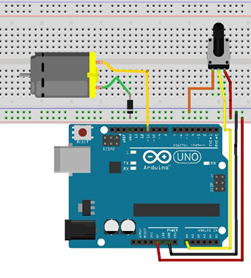
\includegraphics[width=0.8\linewidth]{29. Circuit motor control}
\end{center}

\newpage

\section{Electronics part 2}

\marginfigure{30. Component transistor}

\marginfigure{31. Component transistor pinout}

\marginfigure[0pt][0.8]{32. Component transistor function}

An electric motor can consume a lot of power. The Arduino is bad at providing a lot of power. To provide large power consumers with the necessary power, you can use an external power source such as a battery. Then you still need a transistor so that you can control the magnitude of the current and adjust the speed of rotation of the electric motor.

The transistor (here we only use a so-called NPN transistor) has three legs, see the photo. The emitter is on the left, the base in the middle and the collector on the right. (ATTENTION! With several transistors the pin order is different, we assume you use the 2N222 transistor). The external power supply (+ side) is connected to the collector at all times. Voltage across the base determines whether current will flow to the emitter. This makes a transistor a kind of tap: the amount of voltage at the base determines the amount of current that is passed. The base must therefore be controlled with a PWM pin if you want to control the speed.

With very high currents you have to use a larger transistor or one with a cooling element so that the transistor can lose its heat.

\subsection{Question 14 The speed of an electric motor part 2}

The circuit of assignment 13 is too simple and the Arduino may well be supplying too little current. Especially when you want to run the DC motor quickly.

\begin{alphalist}
\item Build the circuit as shown below.

\item Use the script from assignment 12 and upload the program. Can the electric motor actually turn faster?
\end{alphalist}

\begin{center}
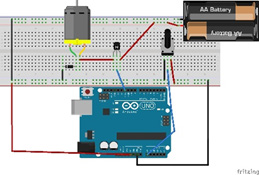
\includegraphics[width=0.8\linewidth]{33. Circuit motor control (large current)}
\end{center}

\newpage

\section{Programming part 4}

\marginfigure[\baselineskip][0.5]{34. Component servo}

Scripts have already been written for controlling some devices, making controlling the devices easier. One of those devices is a servo motor. A servo motor is a type of electric motor that can rotate \ang{180}. The rotation angle can be set precisely because it works with a built-in potentiometer. To use a servo we need the following script.

\begin{lstlisting}
#include <Servo.h>
Servo mijnServo;
int pos = 0;
void setup() {
  mijnServo.attach(9)
}
\end{lstlisting}

First, the script is retrieved from the library. Then we call the servo myServo and it gets the starting position 0.

With \lstinline{myServo.attach (9)} we say that the servo is connected to pin 9. Of course this is another PWM port.

Now it is possible to control the servo. Where pos stands for the position, it can be between 0 and 180. The code for controlling this servo will then be: \lstinline{myServo.write (pos);} A servo motor cannot rotate completely like a normal electric motor, but we can aim very well with a servo motor. This is because there is a potentiometer in the Servo, so the control is done by reading the voltage!

\subsection{Assignment 15 A light measuring device}

Use assignment 8 as a basis. Replace the LED with the servo motor. You can stick a pointer on the servo and make a scale so that the pointer indicates how light / dark it is.

\subsection{Question 16 As much sunlight as possible}

\marginfigure{35. Control light}

Solar panels are installed to convert radiant energy from the sun into electrical energy. The panels receive the most light when they are perpendicular to the sun. The earth rotates and we should let the panels rotate to capture as much energy as possible. We are going to do that in this assignment.

All solar panels are set up on a large field, such as solar panel 1. Solar panel 2 and 3 are both slightly rotated in relation to panel 1. You can now clearly see that the solar panels would produce the most electrical energy if solar panels 2 and 3 would produce the same amount of electrical energy. However, currently panel 2 now captures more light rays than panel 3. So the whole system should be turned counterclockwise.

\newpage

\marginfigure{36. Circuit solar panel control}
Instead of a solar cell, we start with an LDR.

\begin{alphalist}
\item Build the circuit and program the first piece where you can read the values ​​of the LDR.

\item Turn on the flash of your phone and read using \lstinline{Serial.println(LDR1);} the values ​​of LDR 1 and LDR2. Move your phone from left to right and watch the values ​​vary.

\item Now write the piece of code for the servo. Turn the servo to the left if LDR1 receives more light than LDR2 and vice versa. Keep in mind that the servo uses a potentiometer and you can also use the map function.

\item Explain that it is already quite close to rotating the solar panels.
\end{alphalist}

\begin{widebox}
\subsection{Assignment 17 LCD}

With an LCD screen (liquid crystal display) it is possible to print information on a small screen. This eliminates the need to use the serial monitor (and computer) to read data.\vspace{\baselineskip}

\begin{minipage}{\linewidth}\centering
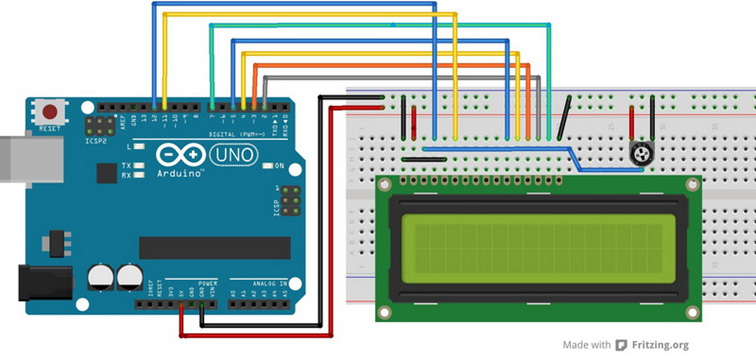
\includegraphics[width=0.7\linewidth]{37. Circuit display}
\end{minipage}

\begin{alphalist}
\item Create the setup shown here.

\item Open the program HelloWorld, it can be found at File / examples / LiquidCrystal and upload the program. Note! With HelloWorld your backlight is not yet on, you can control this using pin 7 (and insert the piece of code). You can also always have the backlight on by not connecting to pin 7 but to the +.

\item Try to read the script and see if you understand what the LCD shows.
\end{alphalist}

The script uses a library. A library is a piece of code written by others, which makes programming a lot easier for you. Libraries have already been made for many different sensors, so it is only a matter of finding them. This often works through, for example: \href{instructables.com}{instructables.com} or \href{arduino.cc}{arduino.cc}. All possible functions for this specific library can be found at: \href{arduino.cc/en/reference/LiquidCrystal}{https://www.arduino.cc/en/reference/LiquidCrystal}

Let's take a look at the script: after reading the library, we should specify the pins that will be used. The setup specifies that the lcd has 16 columns and two rows (\lstinline{lcd.begin(16,2);}). The text hello, world is also immediately printed (everything in the setup is done 1x!).

Over time, the time the Arduino is on (\lstinline{millis ();}) is printed to the LCD, to line 2.

\begin{alphalist}
\item Expand your circuit with a push button and change the code so that the LCD screen shows how many times you pressed the button.
\end{alphalist}
\end{widebox}

\newpage

\section{Functions}

\begin{widebox}
There is a huge list of features. What follows are the most common functions that are used in Arduino.

\newlength{\functionsCOLi}\setlength{\functionsCOLi}{\widthof{\lstinline[]!map(W,Min1,Max1,Min2,Max2)!}}
\begin{longtable}{
    >{\raggedright\arraybackslash}p{\functionsCOLi}
    >{\raggedright\arraybackslash}p{\linewidth-\functionsCOLi-4\tabcolsep}
    }
\toprule
\textbf{Function} & \textbf{Explanation} \\
\midrule
\endhead
\midrule \multicolumn{2}{r}{{\scriptsize\textit{Continues on the next page}}} \\ \bottomrule
\endfoot
\bottomrule
\endlastfoot 
{\lstinline[]!int!} &
value between -32768 en 32767 (215) \\
{\lstinline[]!long!} &
value between -2.147.483.648 en 2.147.483.647 (231) \\
{\lstinline[]!unsigned long!} / {\lstinline[]!unsigned int!} &
only positive values \\
{\lstinline[]!char!} &
characters stored via the ASCII system \\
{\lstinline[]!float!} &
are decimal values, but are avoided as much as possible in Arduino \\
{\lstinline[]!digitalWrite(pin,waarde);!} &
does not write voltage ({\lstinline[]!LOW!}) or a voltage of \SI{5.0}{\volt} to the pin. \\
{\lstinline[]!analogWrite(pin,waarde)!} &
Writes with an 8 bit output values ​​between 0 and \SI{5.0}{\volt}. The indicated value must be between 0 and 255. \\
{\lstinline[]!digitalRead(pin)!} &
reads if there is a voltage on the pin, returns a 0 or 1. \\
{\lstinline[]!analogRead(pin)!} &
reads how much voltage is on the pin, returns a value between 0 and 1023. \\
{\lstinline[]!map(W,Min1,Max1,Min2,Max2)!} &
Is a scaling function. Converts a value ({\lstinline[]!W!}) between {\lstinline[]!Min1!} and {\lstinline[]!Max1!} to a value between {\lstinline[]!Min2!} and {\lstinline[]!Max2!}. \\
{\lstinline[]!if(voorwaarde){}!} &
If the set condition is met, the code between the curly brackets is executed. \\
{\lstinline[]!while(voorwaarde){}!} &
As long as the condition is met, the code between the braces will be executed. \\
{\lstinline[]!for(init;cond;incr){}!} &
A for loop executes the code between the braces a number of times. {\lstinline[]!init!} is the initial value, {\lstinline[]!cond!} is the condition and {\lstinline[]!incr!} is the increment. Ex: {\lstinline[]!for(int i = 0; i<20;i++){delay(100);}!} \\
{\lstinline[]!switch case!} &
switch case is a kind of menu where a piece of code can be executed. If the variable has value one, it executes the code associated with case 1. See code block below.\\
{\lstinline[]!&&!} &
Both conditions must apply \\
{\lstinline[]!||!} &
One of the two conditions must apply \\
{\lstinline[]!!=!} &
Is not equal to. \\
{\lstinline[]!Tone(pin,f,t);!} &
Can produce specific frequency. The tone must indicate on which pin the speaker is located, which frequency must be made and possibly how long the tone must be held. It is not necessary to specify how long the tone should be held. \\
{\lstinline[]!noTone(pin);!} &
Stops the tone that was being produced. \\
{\lstinline[]!millis();!} &
This can serve as a timer. {\lstinline[]!millis();!} indicates the number of milliseconds that the Arduino is on. \\
{\lstinline[]!micros();!} &
Displays the number of microseconds that the Arduino is on. The resolution is \SI{4}{\micro\s}. \\
{\lstinline[]!delay();!} &
Wait a few milliseconds for the next piece of code to run. \\
{\lstinline[]!random(min,max)!} &
Random returns a number between the lowest value ({\lstinline[]!min!}) and highest value ({\lstinline[]!max!}). A disadvantage of random is that the same sequence is played when the Arduino is restarted. Random is not random\dots. This problem can be solved by first using the {\lstinline[]!randomSeed(analogRead(0));!} function. This reads pin A0. If nothing is connected there, noise is measured here. randomSeed shakes up Random's fixed sequence, as it were.\\
\end{longtable}
\end{widebox}

\bigskip

\begin{lstlisting}
switch (var) {
  case 1: \\ do something if var is 1
  break;
  case 2: \\ do something if var is 2
  break;
  default: \\ if neither of the above is true, then do the following (optional)
  break;
}
\end{lstlisting}

\newpage

\section{Attachment: code Blink.ino}

\begin{minipage}{\widemargin}
\begin{lstlisting}
/*
  Blink
  Turns on an LED on for one second, then off for one second, repeatedly.

  Most Arduinos have an on-board LED you can control. On the Uno and
  Leonardo, it is attached to digital pin 13. If you're unsure what
  pin the on-board LED is connected to on your Arduino model, check
  the documentation at http://www.arduino.cc

  This example code is in the public domain.

  modified 8 May 2014
  by Scott Fitzgerald
 */


// the setup function runs once when you press reset or power the board
void setup() {
  // initialize digital pin 13 as an output.
  pinMode(13, OUTPUT);
}

// the loop function runs over and over again forever
void loop() {
  digitalWrite(13, HIGH);   // turn the LED on (HIGH is the voltage level)
  delay(1000);              // wait for a second
  digitalWrite(13, LOW);    // turn the LED off by making the voltage LOW
  delay(1000);              // wait for a second
}
\end{lstlisting}
\end{minipage}

\newpage

\section{Attachment: code Fade.ino}

\begin{minipage}{\widemargin}
\begin{lstlisting}
/*
 Fade

 This example shows how to fade an LED on pin 9
 using the analogWrite() function.

 The analogWrite() function uses PWM, so if
 you want to change the pin you're using, be
 sure to use another PWM capable pin. On most
 Arduino, the PWM pins are identified with 
 a "~" sign, like ~3, ~5, ~6, ~9, ~10 and ~11.

 This example code is in the public domain.
 */

int led = 9;           // the PWM pin the LED is attached to
int brightness = 0;    // how bright the LED is
int fadeAmount = 5;    // how many points to fade the LED by

// the setup routine runs once when you press reset:
void setup() {
  // declare pin 9 to be an output:
  pinMode(led, OUTPUT);
}

// the loop routine runs over and over again forever:
void loop() {
  // set the brightness of pin 9:
  analogWrite(led, brightness);

  // change the brightness for next time through the loop:
  brightness = brightness + fadeAmount;

  // reverse the direction of the fading at the ends of the fade:
  if (brightness == 0 || brightness == 255) {
    fadeAmount = -fadeAmount ;
  }
  // wait for 30 milliseconds to see the dimming effect
  delay(30);
}
\end{lstlisting}
\end{minipage}

\newpage

\section{Attachment: code Button.ino}

\begin{minipage}{\widemargin}
\begin{lstlisting}
/*
  Button

 Turns on and off a light emitting diode(LED) connected to digital
 pin 13, when pressing a pushbutton attached to pin 2.


 The circuit:
 * LED attached from pin 13 to ground
 * pushbutton attached to pin 2 from +5V
 * 10K resistor attached to pin 2 from ground

 * Note: on most Arduinos there is already an LED on the board
 attached to pin 13.


 created 2005
 by DojoDave <http://www.0j0.org>
 modified 30 Aug 2011
 by Tom Igoe

 This example code is in the public domain.

 http://www.arduino.cc/en/Tutorial/Button
 */

// constants won't change. They're used here to
// set pin numbers:
const int buttonPin = 2;     // the number of the pushbutton pin
const int ledPin =  13;      // the number of the LED pin

// variables will change:
int buttonState = 0;         // variable for reading the pushbutton status

void setup() {
  // initialize the LED pin as an output:
  pinMode(ledPin, OUTPUT);
  // initialize the pushbutton pin as an input:
  pinMode(buttonPin, INPUT);
}

void loop() {
  // read the state of the pushbutton value:
  buttonState = digitalRead(buttonPin);

  // check if the pushbutton is pressed.
  // if it is, the buttonState is HIGH:
  if (buttonState == HIGH) {
    // turn LED on:
    digitalWrite(ledPin, HIGH);
  } else {
    // turn LED off:
    digitalWrite(ledPin, LOW);
  }
}
\end{lstlisting}
\end{minipage}

\newpage

\section{Attachment: code AnalogReadSerial.ino}

\begin{minipage}{\widemargin}
\begin{lstlisting}
/*
  AnalogReadSerial
  Reads an analog input on pin 0, prints the result to the serial monitor.
  Graphical representation is available using serial plotter (Tools > Serial Plotter menu)
  Attach the center pin of a potentiometer to pin A0, and the outside pins to +5V and ground.

  This example code is in the public domain.
*/

// the setup routine runs once when you press reset:
void setup() {
  // initialize serial communication at 9600 bits per second:
  Serial.begin(9600);
}

// the loop routine runs over and over again forever:
void loop() {
  // read the input on analog pin 0:
  int sensorValue = analogRead(A0);
  // print out the value you read:
  Serial.println(sensorValue);
  delay(1);        // delay in between reads for stability
}
\end{lstlisting}
\end{minipage}

\end{document}